
\section{Global Presentation of the Library}

\texttt{OpenMotion} est une librairie open source qui. En utilisant uniquement les donnee de l'IMU integre au telephone. La librairie ne supporte pas encore les translations, nous nous sommes concentre sur l'attitude. 


Voici les 2 reference frame utiliser pour la creation de la librairie

\vspace{0.1cm}

\begin{itemize}
\item The North East Down (NED) frame $\{a\}$ system has its origin fixed at the (moving) object center of gravity. The $z$-axis points upward perpendicularly to the tangent plane of the ellipsoid, and the $x$-axis points towards true north (and not the magnetic north). The $y$-axis point towards east.

\vspace{0.1cm}

\item The object-fixed reference frame $\{c\}$ corresponding to the IMU device. It is a moving and rotating coordinate frame. 
\end{itemize}

\vspace{0.1cm}

The library admit admit that all the components of the IMU belong to the same reference frame $\{c\}$ (ref figure\ref{Schema_situation}). It is a cyclopean approximation \cite{ouarti2008multimodal} .

\begin{figure}
\centering
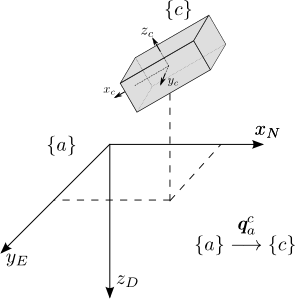
\includegraphics[scale=0.65]{images/Schema_situation.png}
\caption{Definition of the scene with 2 frame:  a fixed frame NED (North East Down) noted $\{a\}$ and a moving frame object noted $\{c\}$}
\label{Schema_situation}
\end{figure}



La librairie permet aussi l'utilisation de different algo de fusion selon le choix de l'interesse. 
Ainsi que le type de sortie (quat, rotation matrix, euler angle, rodriguez etc...)
et elle n'estime que l'orientation par rapport a NED. d'autre transformation sont necessaire pour passer dans d'autre reference frame.




\begin{lstlisting}
// om_exemple.cpp
#include <om.h>

using namespace om;

void main(int argc, char** argv){

	// 
	SensorFusionManager manager;

	//if calibration is necessary
	manager.calibration();
	
	// while IMU send data
	while( isData ){

		// set all IMU data at time t
		manager.setGyroscopeData(gyro_x,gyro_y,gyro_z);	
		manager.setAccelerometerData(acc_x,acc_y,acc_z);
		manager.setMagnetometerData(mag_x,mag_y,mag_z);
		
		// get different kind of output according to user's choices
		
		// quaternion
		Quaternion q_est = manager.getAttitude<Quaternion>(); 
		
		//  rotation matrix
		Matrix R = manager.getAttitude<Matrix>(); 
		
		//  axis angle
		AxisAngle axisAngle = manager.getAttitude<Matrix>(); 
		...
	}
}
\end{lstlisting}

We are also working on the establishment of a dynamic sensor calibration process on all component of the IMU. We insist on the dynamic aspect. Indeed, firstly, it allows  the library to be adaptable to any kind of IMU, but also to improve the performance without requesting some effort from the user.
